\documentclass[10pt]{extarticle}
\title{}
\author{Avinash Iyer}
\date{}
\usepackage[shortlabels]{enumitem}

%font setup
%
%\usepackage{newpxtext,eulerpx}

%paper setup
\usepackage{geometry}
\geometry{letterpaper, portrait, margin=1in}
\usepackage{fancyhdr}

%symbols
\usepackage{amsmath}
\usepackage{amssymb}
\usepackage{mathtools}
\usepackage{hyperref}
\usepackage{gensymb}
\usepackage{multirow,array}

\usepackage[T1]{fontenc}
\usepackage[utf8]{inputenc}

%chemistry stuff
\usepackage[version=4]{mhchem}
\usepackage{chemfig}

%plotting
\usepackage{pgfplots}
\usepackage{tikz}
\tikzset{middleweight/.style={pos = 0.5, fill=white}}
\tikzset{weight/.style={pos = 0.5, fill = white}}
\tikzset{lateweight/.style={pos = 0.75, fill = white}}
\tikzset{earlyweight/.style={pos = 0.25, fill=white}}

%\usepackage{natbib}

%graphics stuff
\usepackage{graphicx}
\graphicspath{ {./images/} }

%code stuff
%when using minted, make sure to add the -shell-escape flag
%you can use lstlisting if you don't want to use minted
%\usepackage{minted}
%\usemintedstyle{pastie}
%\newminted[javacode]{java}{frame=lines,framesep=2mm,linenos=true,fontsize=\footnotesize,tabsize=3,autogobble,}
%\newminted[cppcode]{cpp}{frame=lines,framesep=2mm,linenos=true,fontsize=\footnotesize,tabsize=3,autogobble,}

\usepackage{listings}
%\usepackage{color}
%\definecolor{dkgreen}{rgb}{0,0.6,0}
%\definecolor{gray}{rgb}{0.5,0.5,0.5}
%\definecolor{mauve}{rgb}{0.58,0,0.82}
\lstset{
  breaklines = true,
  basicstyle = \small\ttfamily
}
%\lstset{frame=tb,
%	language=Java,
%	aboveskip=3mm,
%	belowskip=3mm,
%	showstringspaces=false,
%	columns=flexible,
%	basicstyle={\small\ttfamily},
%	numbers=none,
%	numberstyle=\tiny\color{gray},
%	keywordstyle=\color{blue},
%	commentstyle=\color{dkgreen},
%	stringstyle=\color{mauve},
%	breaklines=true,
%	breakatwhitespace=true,
%	tabsize=3
%}
% text + color boxes
\usepackage[most]{tcolorbox}
\tcbuselibrary{breakable}
\newtcolorbox{problem}[1]{colback = white, title = {#1}, breakable}
\newtcolorbox{solution}{colback = white, colframe = black!75!white, title = Solution, breakable}
%including PDFs
%\usepackage{pdfpages}
\setlength{\parindent}{0pt}

\pagestyle{fancy}
\fancyhf{}
\rhead{Avinash Iyer}
\lhead{Math 300: Homework 2}
\newcommand{\card}{\text{card}}
\newcommand{\ran}{\text{ran}}
\newcommand{\N}{\mathbb{N}}
\newcommand{\Q}{\mathbb{Q}}
\newcommand{\Z}{\mathbb{Z}}
\newcommand{\R}{\mathbb{R}}
\begin{document}
  \begin{problem}{Problem 1}
    \begin{lstlisting}
      % Problem 1
      A = [0 1 5 3 4 5 7 9 10]
      (2/3) * A - 4
    \end{lstlisting}
  \end{problem}
  \begin{problem}{Problem 2}
    \begin{lstlisting}
      % Problem 2
      t = 1:10
      x = t.*sin(t)
      y = (t-1)./(t+1)
      z = sin(t.^2)./t.^2
    \end{lstlisting}
  \end{problem}
  \begin{problem}{Problem 3}
    \begin{lstlisting}
      % Problem 3
      A = rand(4,3)
      A(3:4,2:3)
      A = [A(:,1) A(:,2) A(:,3) A(:,1)]
      A(2:4,2:4) = eye(3)
      A = [A(1,:);A(3,:)]
      round(A)
      A(:)'
    \end{lstlisting}
  \end{problem}
  \begin{problem}{Problem 4}
    \begin{lstlisting}
      % Problem 4
      v=0:0.2:12;
      M=[sin(v);cos(v)];
      size(M)
      size(v)
      M(:,1:10)'
    \end{lstlisting}
  \end{problem}
  \begin{problem}{Problem 5}
    \begin{lstlisting}
      % Problem 5
      x=0:pi/100:2*pi;
      y1=sin(x);
      y2=cos(x);
      y3=tan(x);

      plot(x,y1,x,y2,x,y3)
      ylim([-2 2]);
      legend('sin(x)','cos(x)','tan(x)')
      title('Graph 1')
      xlabel('x')
      ylabel('y')
    \end{lstlisting}
    \begin{center}
      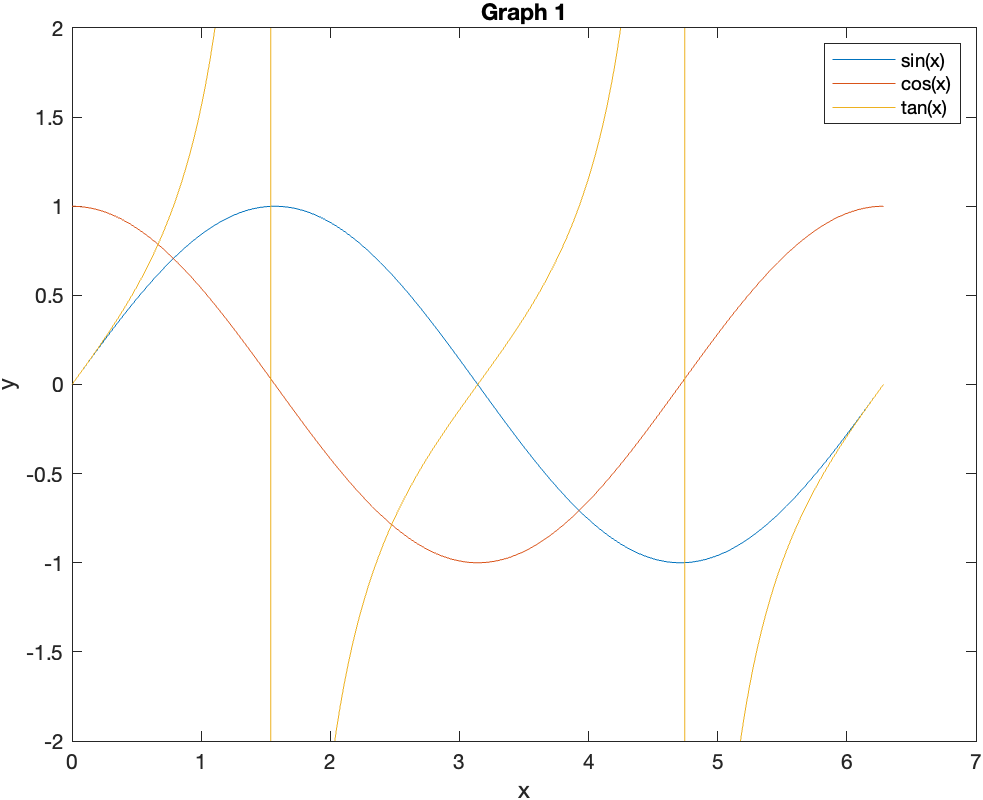
\includegraphics[width=10cm]{problem_5}
    \end{center}
  \end{problem}
  \begin{problem}{Problem 6}
    \begin{lstlisting}
      % Problem 6
      syms t
      f = diff(sin(t));
      x=0:pi/100:2*pi;
      y1=sin(x);
      y2=vpa(subs(f,t,2))*(x-2) + sin(2);
      plot(x,y1,x,y2);
      ylim([-2 2]);
      legend('sin(x)','tangent line at x=2')
      title('Graph 2')
      xlabel('x')
      ylabel('y')
    \end{lstlisting}
    \begin{center}
      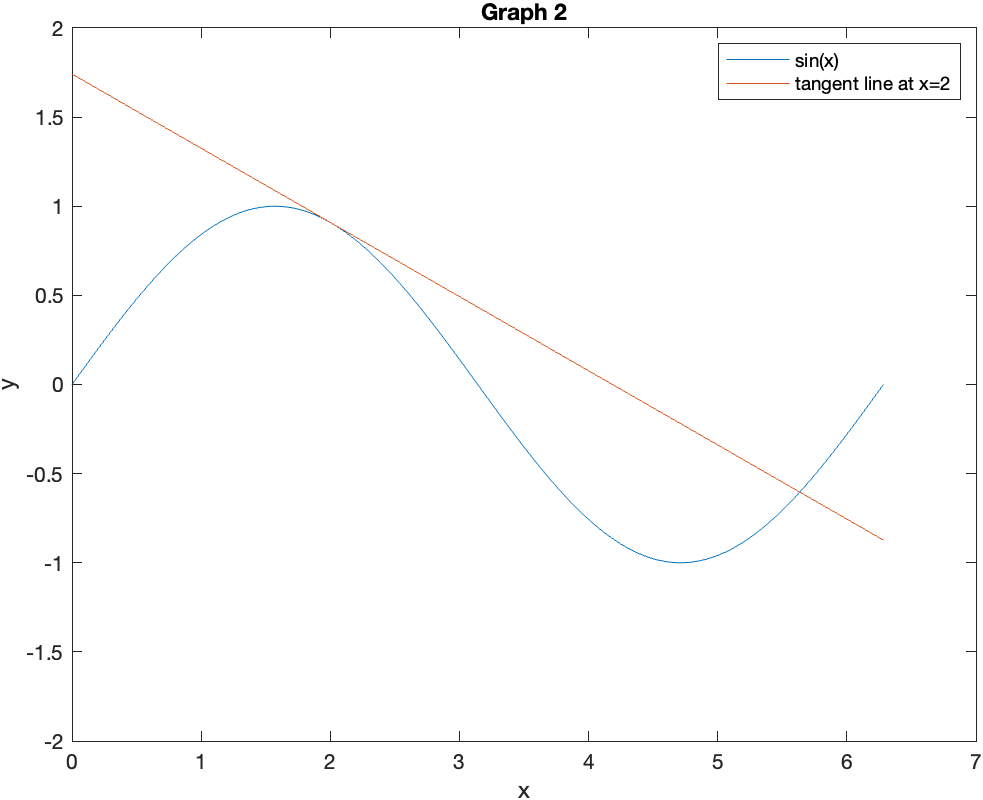
\includegraphics[width=10cm]{problem_6}
    \end{center}
  \end{problem}
  \begin{problem}{Command Line Output}
    \begin{lstlisting}
      >> problem_1

      A =

           0     1     5     3     4     5     7     9    10


      ans =

         -4.0000   -3.3333   -0.6667   -2.0000   -1.3333   -0.6667    0.6667    2.0000    2.6667

      >> problem_2

      t =

           1     2     3     4     5     6     7     8     9    10


      x =

          0.8415    1.8186    0.4234   -3.0272   -4.7946   -1.6765    4.5989    7.9149    3.7091   -5.4402


      y =

               0    0.3333    0.5000    0.6000    0.6667    0.7143    0.7500    0.7778    0.8000    0.8182


      z =

          0.8415   -0.1892    0.0458   -0.0180   -0.0053   -0.0275   -0.0195    0.0144   -0.0078   -0.0051

      >> problem_3

      A =

          0.9572    0.4218    0.6557
          0.4854    0.9157    0.0357
          0.8003    0.7922    0.8491
          0.1419    0.9595    0.9340


      ans =

          0.7922    0.8491
          0.9595    0.9340


      A =

          0.9572    0.4218    0.6557    0.9572
          0.4854    0.9157    0.0357    0.4854
          0.8003    0.7922    0.8491    0.8003
          0.1419    0.9595    0.9340    0.1419


      A =

          0.9572    0.4218    0.6557    0.9572
          0.4854    1.0000         0         0
          0.8003         0    1.0000         0
          0.1419         0         0    1.0000


      A =

          0.9572    0.4218    0.6557    0.9572
          0.8003         0    1.0000         0


      ans =

           1     0     1     1
           1     0     1     0


      ans =

          0.9572    0.8003    0.4218         0    0.6557    1.0000    0.9572         0

      >> problem_4

      ans =

           2    61


      ans =

           1    61


      ans =

               0    1.0000
          0.1987    0.9801
          0.3894    0.9211
          0.5646    0.8253
          0.7174    0.6967
          0.8415    0.5403
          0.9320    0.3624
          0.9854    0.1700
          0.9996   -0.0292
          0.9738   -0.2272

      >> problem_5
      >> problem_6
    \end{lstlisting}
  \end{problem}
\end{document}
